\documentclass[11pt]{article}

\usepackage[utf8]{inputenc}
\usepackage[spanish, es-tabla]{babel}
\usepackage{mathtools}
\usepackage{amssymb}
\usepackage{amsthm} 
\usepackage{graphicx}
\usepackage{dsfont}

%Gummi|065|=)
\title{\textbf{Ejemplos}}
\author{Pedro Bonilla Nadal\\
		Johanna Capote Robayna\\
		Guillermo Galindo Ortuño}
\date{}

%No indent
\setlength\parindent{0pt}
\begin{document}

\maketitle
\section*{Ejercicio 2} 
\underline{Datos} 
\begin{itemize}
\item $f = log(x)$ 
\item $a = 1, b=2$
\item $ n = 5$

\end{itemize}

\underline{Solución} \\
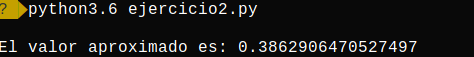
\includegraphics[width=0.7\textwidth]{../images/dos_1} \\
\section*{Ejercicio 3}
\underline{Datos}
\begin{itemize}
\item $f = log(x)$ 
\item $a = 1, b=2$
\item $ n = 200$

\end{itemize}

\underline{Solución} \\
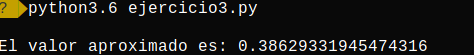
\includegraphics[width=0.7\textwidth]{../images/tres_1}


\section*{Ejercicio 5}
\underline{Datos}
\begin{itemize}
\item $f = log(x)$ 
\item $a = 1, b=2$
\item $ n = 10$

\end{itemize}

\underline{Solución} \\
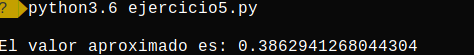
\includegraphics[width=0.7\textwidth]{../images/cinco_1} \\





\end{document}
